

\chapter{Implementazione della paginazione}

\section{Extra: \emph{typedef} per indirizzi fisici e virtuali} Nel file \emph{tipo.h} della \emph{libce} sono presenti due ulteriori typedef per distinguere indirizzi fisici da indirizzi virtuali (solo comodità visiva, sono entrambi \emph{unsigned long})!
\begin{itemize}
	\item \begin{verbatim}typedef unsigned long vaddr;\end{verbatim}
	Indirizzi virtuali
	\item \begin{verbatim}typedef unsigned long paddr;\end{verbatim}
	Indirizzi fisici
\end{itemize}
Sono molto utilizzati nelle funzioni di \emph{vm.h}. In quest'ultimo file troviamo anche 
\begin{itemize}
	\item \begin{verbatim}typedef natq tab_entry;
	\end{verbatim}
	che usiamo per le entrate delle tabelle delle pagine.
\end{itemize} 
\section{Costanti in \emph{vm.h} della \emph{libce}}
\subsection{Numero massimo di livelli del \emph{trie}} \begin{verbatim}
	static const int MAX_LIV = 4;
\end{verbatim}
Numero di livelli massimo. Nel nostro codice abbiamo $4$, ma con processori a $57$ bit è possibile avere un livello in più. 
\subsection{Maschere}
\begin{itemize}
	\item 
	\begin{verbatim}
		static const natq BIT_SEGNO = (1ULL << (12 + 9* MAX_LIV -1)); <- ULL unsigned long long
	\end{verbatim}
	Calcoliamo il bit dove si trova il segno (l'ultimo bit più significativo che ci interessa). Si pone ULL per evitare problemi con lo shift. La maschera è utile nella funzione per la normalizzazione degli indirizzi. Nel caso nostro avremo:
	\begin{verbatim}
		BIT_SEGNO = (1ULL << 47);
	\end{verbatim}
	\item \begin{verbatim} 
		static const natq MASCHERA_MODULO = BIT_SEGNO - 1;
	\end{verbatim} 
	Maschera con cui recupero il modulo.
\end{itemize}	
\subsection{Costanti per la manipolazione dei descrittori di pagina e di tabella}
\small
\begin{verbatim}
	const natq BIT_P    = 1U << 0; // il bit di presenza
	const natq BIT_RW   = 1U << 1; // il bit di lettura/scrittura
	const natq BIT_US   = 1U << 2; // il bit utente/sistema
	const natq BIT_PWT  = 1U << 3; // il bit Page Wright Through
	const natq BIT_PCD  = 1U << 4; // il bit Page Cache Disable
	const natq BIT_A    = 1U << 5; // il bit di accesso
	const natq BIT_D    = 1U << 6; // il bit "dirty"
	const natq BIT_PS   = 1U << 7; // il bit "page size"
	
	const natq ACCB_MASK  = 0x00000000000000FF; // maschera per il byte di accesso
	const natq ADDR_MASK  = 0x7FFFFFFFFFFFF000; // maschera per l'indirizzo
\end{verbatim}
\normalsize

\section{Funzioni in \emph{vm.h} della \emph{libce}}
Il file è incluso attraverso apposita direttiva in \emph{sistema.cpp}, precisamente nella sezione dedicata alla paginazione
\begin{verbatim}
	#include <vm.h>
\end{verbatim}
\subsection{Normalizzazione dell'indirizzo con \emph{norm}}
\small 
\begin{verbatim}
	static inline vaddr norm(vaddr a) {
		return (a & BIT_SEGNO) ? (a | ~MASCHERA_MODULO) : (a & MASCHERA_MODULO);
	}
\end{verbatim}
\normalsize 
%\begin{center}
%	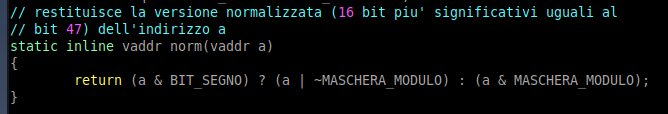
\includegraphics{img/236.PNG}
%\end{center} 
\begin{itemize}
	\item Dato un indirizzo virtuale la funzione restituisce la corrispondente versione normalizzata (i $16$ bit più significativi sono uguali al $47-$esimo bit dell'indirizzo).
	\item Step:
	\begin{itemize}
		\item Controlliamo il bit di segno.
		\item Se è uguale ad $1$ metto i bit più significativi rimanenti uguali ad $1$
		\item Se è uguale a 0 metto  i bit più significativi rimanenti uguali a $0$.
	\end{itemize}
\end{itemize}
\subsection{Grandezza di una regione con \emph{dim$\_$region}}
\small 
\begin{verbatim}
	static inline constexpr natq dim_region(int liv) {
		natq v = 1ULL << (liv * 9 + 12);
		return v;
	}
\end{verbatim}
\normalsize 
%\begin{center}
%	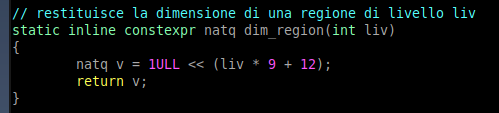
\includegraphics{img/237.PNG}
%\end{center} 
\paragraph{Definizione} Con \emph{regione di livello liv} intendiamo l'intervallo di indirizzi coperti da una singola entrata di una tabella di livello $i+1$. Questo significa che:
\begin{itemize}
	\item una regione di livello $0$ è grande $4096\,\text{byte}$;
	\item una regione di livello $1$ è grande $2\,\text{MiB}$;
	\item una regione di livello $3$ è grande $1\,\text{GiB}$.
\end{itemize}
\paragraph{Scopo della funzione} La funzione ci restituisce la grandezza di una regione di livello \emph{liv}: prendo $12$ (numero di bit dell'offset) e mi ricordo che ogni livello è rappresentato da $9$ bit, quindi sommo a $12$ il prodotto tra $9$ e \emph{liv}. Concludiamo traslando
\[1 \cdot 2^{\text{liv} \cdot 9 + 12}\]

\subsection{Funzioni \emph{base} e \emph{limit} per l'indirizzo di base di una regione}
\small 
\begin{verbatim}
	static inline vaddr base(vaddr v, int liv) {
		natq mask = dim_region(liv) - 1;
		return v & ~mask;
	}
	
	static inline vaddr limit(vaddr e, int liv) {
		natq dr = dim_region(liv);
		natq mask = dr - 1;
		return (e + dr - 1) & ~mask;
	}
\end{verbatim}
\normalsize 
%\begin{center}
%	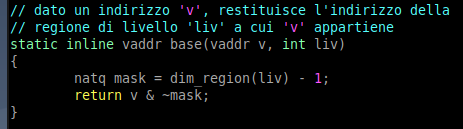
\includegraphics{img/238.PNG}
%\end{center} 
%\begin{center}
%	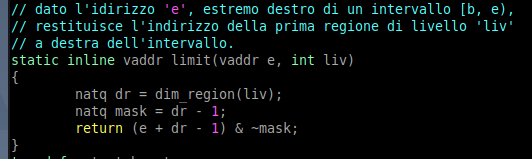
\includegraphics{img/239.PNG}
%\end{center} 
Dato un indirizzo virtuale \emph{v} le due funzioni restituiscono un altro indirizzo virtuale. Precisamente:
\begin{itemize}
	\item la funzione \emph{base} restituisce la base della pagina di livello \emph{liv} in cui cade l'indirizzo \emph{v};
	\begin{itemize}
		\item Otteniamo il numero di regione mascherando i bit meno significativi dell'indirizzo. Vediamo un esempio semplificato
		\[0b1000 - 0b0001 = 0b0111 \longrightarrow \,!(0b0111)=0b1000\]
		Se uso l'operatore AND spariscono i tre bit meno significativi.
	\end{itemize}
	\item la funzione \emph{limit} restituisce la base della prima regione di livello \emph{liv} a destra dell'intervallo (quello della regione dove si trova l'indirizzo \emph{v}).
	\begin{itemize}
		\item Recupero la dimensione di una regione di livello \emph{liv}.
		\item  Decremento per ottenere una maschera (bit più significativo uguale a $0$, tutti gli altri uguali ad $1$).
		\item Sommo all'indirizzo \emph{e} la dimensione della regione e decremento di $1$. A quel punto faccio AND con la negazione della maschera \emph{mask} (mi sbarazzo dei bit meno significativi).
	\end{itemize}
\end{itemize}

\subsection{Funzioni per lavorare sul \emph{trie}}

\subsubsection{Estrazione dell'indirizzo fisico da un'entrata (\emph{extr$\_$IND$\_$FISICO})}
\small 
\begin{verbatim}
	static inline paddr extr_IND_FISICO(tab_entry descrittore) {
		return descrittore & ADDR_MASK;
	}
\end{verbatim}
\normalsize 
%\begin{center}
%	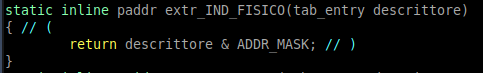
\includegraphics{img/240.PNG}
%\end{center} 
La funzione mi permette di ottenere l'indirizzo fisico presente nella \emph{tab$\_$entry} indicata nei parametri di ingresso. Nel caso della foglia non restituiremo solo un indirizzo fisico, ma l'indirizzo della base del frame.
\paragraph{Cosa faccio} Mi ricordo dove è collocato l'indirizzo fisico all'interno del descrittore, tenendo conto che l'offset (i primi $12$ bit) è sempre una sequenza di zeri. Utilizzo la costante \emph{ADDR$\_$MASK}, già vista
\begin{verbatim}
	const natq ADDR_MASK  = 0x7FFFFFFFFFFFF000;
\end{verbatim}
\subsubsection{Settaggio dell'indirizzo fisico in un'entrata (\emph{set$\_$IND$\_$FISICO})}
\small 
\begin{verbatim}
	static inline void set_IND_FISICO(tab_entry& descrittore, paddr ind_fisico) {
		descrittore &= ~ADDR_MASK;
		descrittore != ind_fisico & ADDR_MASK;
	}
\end{verbatim}
\normalsize 
%\begin{center}
%	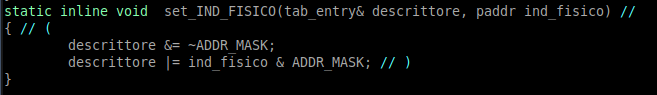
\includegraphics{img/241.PNG}
%\end{center} 
Setto l'indirizzo fisico nel descrittore con due step:
\begin{itemize}
	\item resetto tutti i bit relativi all'indirizzo fisico;
	\item imposto i bit ponendo il nuovo indirizzo fisico (metto l'indirizzo nel descrittore con un OR, dopo aver rimosso l'offset con l'AND).
\end{itemize}
Anche qua utilizziamo la costante \emph{ADDR$\_$MASK}
\begin{verbatim}
	const natq ADDR_MASK  = 0x7FFFFFFFFFFFF000;
\end{verbatim}

\subsubsection{Indice dell'entrata di un vaddr in una tabella di livello \emph{liv}	 (\emph{i$\_$tab})}
\small 
\begin{verbatim}
	static inline int i_tab(vaddr ind_virt, int liv) {
		int shift = 12 + (liv - 1) * 9;
		natq mask = 0x1ffULL << shift;
		return (ind_virt & mask) >> shift;
	}
\end{verbatim}
\normalsize 
%\begin{center}
%	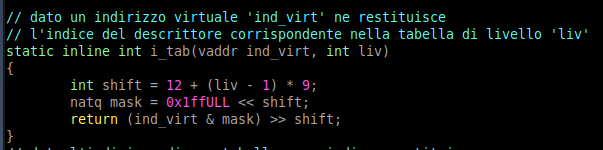
\includegraphics{img/242.PNG}
%\end{center} 
Dato un indirizzo virtuale \emph{ind$\_$virt}, estraggo dall'indirizzo virtuale l'indice del descrittore relativo, in una tabella di livello \emph{liv}.
\begin{itemize}
	\item Prendo una maschera di $9$ bit, che shifto in modo da posizionarla sotto l'indice che mi interessa.
	\item Applico la maschera con l'operatore AND e shifto nuovamente per portare l'indice sulle cifre meno significative.
\end{itemize}

\subsubsection{Indirizzo di un'entrata di indice \emph{index} da una tabella \emph{tab} (\emph{get$\_$entry})}
\small
\begin{verbatim}
	static inline tab_entry& get_entry(paddr tab, natl index) {
		tab_entry *pd = reinterpret_cast<tab_entry*>(tab);
		return pd[index];
	}
\end{verbatim}
\normalsize 
%\begin{center}
%	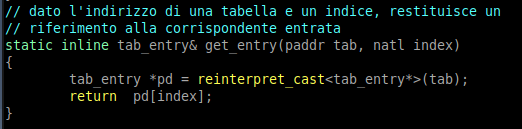
\includegraphics{img/243.PNG}
%\end{center} 
Dato l'indirizzo fisico di una tabella \emph{tab} e un indice \emph{index}, la funzione restituisce il riferimento a una certa entrata.

\subsubsection{Classe \emph{tab$\_$iter} per la visione del trie (iteratore)}
Una cosa che si deve fare molto spesso è visitare l'albero. Uno, per esempio, potrebbe essere interessato a visitare tutte le entrate che si occupano della traduzione degli indirizzi in un certo intervallo di indirizzi. Le strade possibili sono due:
\begin{enumerate}
	\item scrivere una funzione ricorsiva;
	\item realizzare un \emph{iteratore} (cioè un qualcosa che si ricorda in che punto siamo arrivati nell'albero, e rimane lì finchè qualcuno non gli dice di spsotarsi).
\end{enumerate}
{La scelta adottata è la seconda}.
\paragraph{Codice}
\small
\begin{verbatim}
	class tab_iter {
		struct stack {
			vaddr cur, end;
			paddr tab;
		} s[MAX_LIV + 1];
		
		int l;
		
		stack *sp() { return &s[l - 1]; }
		stack const *sp() const { return &s[l - 1]; }
		stack *sp(int lvl) { return &s[lvl - 1]; }
		stack *pp() { return &s[MAX_LIV]; }
		bool done() const { return !sp()->tab; }
		
		public:
		static bool valid_interval(vaddr beg, natq dim) {
			vaddr end = beg + dim - 1;
			return !dim || (
			// no wrap-around
			!(end < beg)
			// non inizia nel buco
			&&   norm(beg) == beg
			// non termina nel buco
			&&   norm(end) == end
			// non attraversa il buco
			&&   !((beg & BIT_SEGNO) != (end & BIT_SEGNO)));
		}
		
		tab_iter(paddr tab, vaddr beg, natq dim = 1, int liv = MAX_LIV);
		
		vaddr get_v() const {
			return sp()->cur;
		}
		
		[... vedere le spiegazioni successive]
		bool down();
		bool up();
		bool right();
		void post();
		void next_post();
	};
\end{verbatim} 
\normalsize
\begin{itemize}
	\item L'iteratore viene costruito indicando:
	\begin{itemize}
		\item l'indirizzo fisico della tabella \emph{tab} (normalmente una tabella di livello $4$), 
		\item un indirizzo virtuale di partenza \emph{beg}  (di cui si vuole visitare la traduzione),
		\item quanto è grande l'intervallo di indirizzi virt. che si vuole visitare (\emph{dim}, di default $1$),
		\item il livello di partenza (di default \emph{MAX$\_$LIV}).
	\end{itemize} 
	\begin{verbatim}
		tab_iter(paddr tab, vaddr beg, natq dim = 1, int liv = MAX_LIV);
	\end{verbatim}
	\item L'operatore booleano indica "se la visita è finita", cioè se tutte le entrate coinvolte nella traduzione che va da \emph{beg} a \emph{beg + DIM} (quest'ultimo escluso) sono state visitate.
	\begin{verbatim}
		bool done() const { return !sp()->tab; }
		operator bool() const {
			return !done();
		}
	\end{verbatim}
	\item Con la funzione \emph{next} indichiamo all'iteratore di spostarsi sulla prossima entrata da visitare. Il tipo di visita è  \emph{anticipata}.
	\begin{verbatim}
		void next();
	\end{verbatim}
	\item Quando siamo fermi su un'entrata possiamo chiedere varie informazioni:
	\begin{itemize}
		\item a che livello siamo
		\begin{verbatim}
			int get_l() const {
				return l;
			}
		\end{verbatim}
		\item se l'entrata è una foglia (ho $P=0$, ho livello $1$, oppure $PS$ è settato)
		\begin{verbatim}
			bool is_leaf() const {
				tab_entry e = get_e();
				return !(e & BIT_P) || (e & BIT_PS) || l == 1;
			}
		\end{verbatim}
		\item il riferimento all'entrata (in modo da poterlo modificare)
		\begin{verbatim}
			tab_entry& get_e() const {
				return get_entry(sp()->tab, i_tab(sp()->cur, l));
			}
		\end{verbatim}
		\item l'indirizzo fisico della tabella che contiene l'entrata su cui l'iteratore è fermo 
		\begin{verbatim}
			paddr get_tab() const {
				return sp()->tab;
			}
		\end{verbatim}
	\end{itemize}
\end{itemize}
\subsubsection{Esempio di uso della classe \emph{tab$\_$iter}} 
Partiamo dalla radice del nostro albero, \emph{tab4} (paddr), e scorre tutto l'intervallo che abbiamo mappato ($8\,\text{MB}$, da $0$ a $0x800000$).
\begin{verbatim}
	for(tab_iter it((paddr)tab4, 0, 0x800000); it; it.next()) {
		flog(LOG_DEBUG, "tab %x, liv %d, entry %x", it.get_tab(), it.get_l(), it.get_e());
	}
\end{verbatim}
L'output è il seguente
\begin{center}
	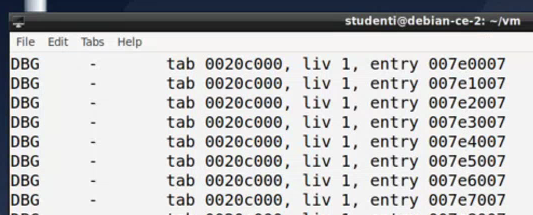
\includegraphics[scale=.85]{img/244.PNG}
\end{center} 
Si includa anche un richiamo alla funzione \emph{panic}, che non fa niente.
\begin{verbatim}
	extern "C" void panic();
\end{verbatim}

\normalsize 

\begin{framed}
	\noindent \textbf{Recap}. Il modulo sistema si deve preoccupare di gestire sia la memoria fisica che quella virtuale.
	\begin{itemize}
		\item \textbf{Memoria fisica}.
		
		Per quanto riguarda quella fisica (la RAM) abbiamo detto che una parte è ad uso esclusivo del modulo sistema (con sezioni \textit{text, data, stack, heap} del sistema), mentre la parte rimanente è divisa in frame. Si tenga conto che tutto ciò che è presente in questa seconda area di memoria non è tutta accessibile all'utente: gli indirizzi devono essere tradotti.
		\item \textbf{Memoria virtuale}.
		
		Il sistema deve creare gli spazi di indirizzamento di ogni singolo processo: abbiamo una serie di indirizzi (col solito buco). A priori decidiamo che tutti gli indirizzi che vanno da $0$ fino al buco appartengono al sistema (solo traduzioni con $U/S=0$, quindi accessibili solo se ci troviamo a livello sistema). La parte rimanente è accessibile a livello utente, contiene traduzioni utilizzabili a livello utente (e anche a livello sistema).
	\end{itemize}
\end{framed}

\clearpage 

\section{Suddivisione dello spazio di indirizzamento}
\paragraph{Sistema} La parte accessibile a livello sistema si divide in tre parti, ciascuna dedicata a priori a una certa cosa:
\begin{itemize}
	\item una prima parte dedicata al \textit{modulo sistema} (unica parte con traduzione identità);
	\item una dedicata al \textit{modulo I/O};
	\item una dedicata alla \textit{pila sistema} (quella usata dal processore a livello sistema).
\end{itemize}
Nel modulo sistema garantiamo all'accesso a tutta la RAM, ma anche ad altre cose come l'APIC. Tutto il resto (modulo I/O, pila sistema e livello utente) conterrà traduzioni che portano ad $M2$.
\paragraph{Utente}
Il livello utente si divide in due parti:
\begin{itemize}
	\item l'area con \emph{text, data, heap};
	\item pila utente.
\end{itemize}
Le pagine sono mappate sempre in $M2$.
\begin{center}
	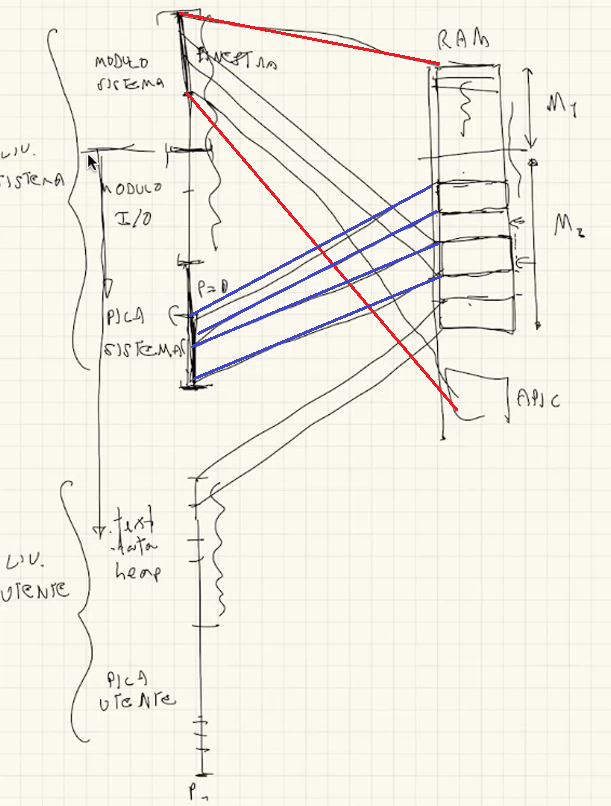
\includegraphics[scale=.6]{img/245.PNG}
\end{center}
\paragraph{Sono necessarie le traduzioni di modulo I/O e pila sistema?} 
\begin{itemize}
	\item Teoricamente non ci sarebbe bisogno di fare queste traduzioni: potrei utilizzare gli indirizzi della finestra, cioè quelli del modulo sistema.
	\item Conviene avere questa seconda traduzione. Abbiamo frame allocati dinamicamente: se il sistema ha già lavorato per un po' diventa molto improbabile che i frame relativi a un processo siano tutti consecutivi. Il mapping per pila e periferiche I/O permette di creare indirizzi contigui (anche se i frame non lo sono). 
\end{itemize} 






\paragraph{Processi concorrenti, mappaggio comune}
Pensiamo a un altro processo, anche lui con la sua memoria virtuale. Alcune traduzioni saranno esattamente identiche a quelle di $P1$:
\begin{itemize}
	\item modulo sistema
	\item modulo I/O
	\item \textit{text, data, heap} del livello utente (gli indirizzi sono gli stessi, ma hanno significato diverso a seconda del processo attivo\footnote{Quindi a seconda della traduzione attiva.}).
\end{itemize}
\paragraph{Attenzione} Alcune persone dicono all'esame che la MMU sceglie se usare la parte sopra o quella sotto in base al livello di privilegio. \textbf{Questa frase non ha alcun senso}: la MMU usa le traduzioni in base agli indirizzi ricevuti e controlla se il livello di privilegio è sufficiente per determinare l'accessibilità della traduzione. Non è un discorso di scegliere cosa usare.

%\paragraph{Cosa dobbiamo sapere?} L'utente, ribadiamo, non ha bisogno di sapere tante cose per scrivere un programma. Nel sistema, invece, dobbiamo ricordare:
%\begin{itemize}
%	\item dove si trova il codice che stiamo leggendo;
%	\item quali indirizzi stiamo usando;
%	\item quali sono le traduzioni attive al momento in cui il codice è stato eseguito.
%\end{itemize}
%Vediamo un esempio in cui è importante sapere queste cose.
%\paragraph{Scrivere nella pila sistema di un altro processo} Sia $P1$ il processo in esecuzione: esso invoca una primitiva di sistema che vuole scrivere qualcosa sulla pila sistema del processo $P2$. Come facciamo?
%\begin{itemize}
%	\item La prima cosa di cui siamo certi è che non utilizzeremo gli indirizzi virtuali della pila sistema, che riguardano il processo in esecuzione $P1$.
%\end{itemize}


\section{Costanti dedicate alla memoria virtuale}
Ritorniamo nel file \emph{include/costanti.h} per vedere alcune costanti legati alla memoria virtuale. Abbiamo detto che la suddivisione dello spazio di indirizzamento in varie parti è fatta a priori. La memoria virtuale è allocata in unità di regioni di livello $4$ (di $512\,\text{GB}$ alla volta). In sostanza decidiamo quante entrate della tabella di livello $4$ di ciascun processo sono dedicate a una cosa oppure a un'altra.
\begin{verbatim}
	// tipo del driver del timer (priorità massima)
	#define TIPO_TIMER		0xFF
	
	// ( suddivisione della memoria virtuale
	//   N    = Numero di entrate in root_tab
	//   I	  = Indice della prima entrata in root_tab
	//   SIS  = SIStema
	//   MIO  = Modulo IO
	//   UTN  = modulo UTeNte
	//   C    = Condiviso
	//   P    = Privato
	#define I_SIS_C		0
	#define I_SIS_P		1
	#define I_MIO_C		2
	#define I_UTN_C       256
	#define I_UTN_P	      384
	
	#define N_SIS_C		1
	#define N_SIS_P		1
	#define N_MIO_C		1
	#define N_UTN_C	      128
	#define N_UTN_P	      128 
	// )
\end{verbatim}
%\begin{center}
%	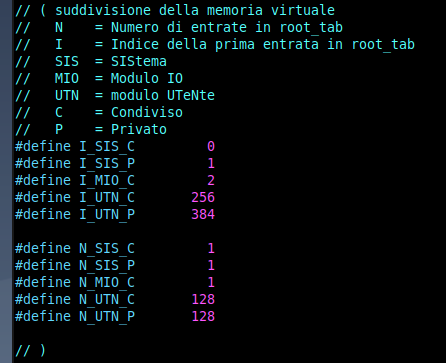
\includegraphics[scale=.9]{img/246.PNG}
%\end{center}
\begin{itemize}
	\item Per ogni parte abbiamo la costante che indica l'entrata iniziale e quella che indica il numero di pagine/frame dedicati alla parte.
	\item \textbf{Esempi}:
	\begin{itemize}
		\item \begin{verbatim}
			#define I_SIC_C    0
			#define N_SIC_C    1
		\end{verbatim}
		\emph{L'entrata iniziale della parte sistema condivisa è la $0$, il numero di entrate dedicato alla parte è $1$}
		\item \begin{verbatim}
			#define I_UTN_C    256
			#define N_UTN_C    128
		\end{verbatim}
		\emph{L'entrata iniziale della parte utente condivisa è la $256$, il numero di entrate dedicato alla parte è $128$}
	\end{itemize}
	\item Si consideri che con \emph{parte sistema privata} si intende la \emph{pila sistema}. Si osservi anche il salto che avviene tra la parte dedicata al modulo I/O e la \emph{parte utente condivisa} (si vuole superare il buco, utilizzando questo per dividere ciò che è rivolto al sistema e ciò che è rivolto all'utente.)
\end{itemize}

\section{Costanti dedicate alla memoria fisica}
Rimaniamo nel file \emph{include/costanti.h}: sono presenti delle costanti dedicate alla memoria fisica.
\small 
\begin{verbatim}
	// ( varie dimensioni
	#define KiB			1024UL
	#define MiB			(1024*KiB)
	#define GiB			(1024*MiB)
	#define DIM_PAGINA		4096UL
	#define DIM_BLOCK		512UL
	// )
	
	// ( limiti modificabili
	// ...
	// dimensione della memoria fisica
	#define MEM_TOT			(32*MiB)
	// dimensione dello heap utente
	#define DIM_USR_HEAP		(1*MiB)
	// dimensione degli stack utente
	#define DIM_USR_STACK		(64*KiB)
	// dimensione dello heap del modulo I/O
	#define DIM_IO_HEAP		(1*MiB)
	// dimensione degli stack sistema
	#define DIM_SYS_STACK		(4*KiB)
	// ...
	// )
\end{verbatim}
\normalsize 
%\begin{center}
%	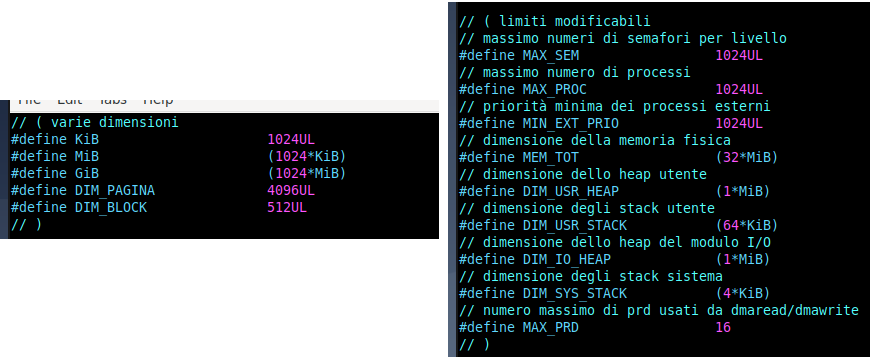
\includegraphics[scale=.9]{img/247.PNG}
%\end{center}
\begin{itemize}
	\item Per prima cosa abbiamo una serie di costanti con cui rappresentiamo le varie unità di misura: \emph{KiB}, \emph{MiB}, \emph{GiB}, \emph{DIM$\_$PAGINA} e \emph{DIM$\_$BLOCK}.
	\item Attraverso altre costanti indichiamo:
	\begin{itemize}
		\item la dimensione della memoria fisica (\emph{MEM$\_$TOT});
		\item la dimensione dello heap utente (\emph{DIM$\_$USR$\_$HEAP});
		\item la dimensione delle pile utente (\emph{DIM$\_$USR$\_$STACK});
		\item la dimensione dello heap del modulo I/O (\emph{DIM$\_$IO$\_$HEAP});
		\item la dimensione delle pile sistema (\emph{DIM$\_$SYS$\_$STACK}).
	\end{itemize}
	\item Le cose indicate sono tutte dimensioni fisiche. Nello spazio fisico le modifiche hanno un costo: ogni cosa dovrà finire da qualche parte, e dovremo fare le corrispondenti traduzioni.
\end{itemize}

\section{Descrittore di processo}
Riprendiamo il descrittore di processo in \emph{sistema/sistema.cpp}. 
\small 
\begin{verbatim}	
	struct des_proc {
		natw id;
		natw livello;
		natl precedenza;
		vaddr punt_nucleo; /* Puntatore a pila sistema */
		natq contesto[N_REG];
		paddr cr3;
		
		des_proc *puntatore;
	};
\end{verbatim}
\normalsize 
%\begin{center}
%	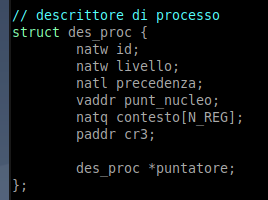
\includegraphics[scale=.85]{img/248.PNG}
%\end{center}
Ogni processo si ricorda l'indirizzo della sua tabella di livello $4$ (\emph{cr3}). 
\section{Aggiornamento del registro CR3 nella \emph{carica$\_$stato}} Una parte del codice della funzione \emph{carica$\_$stato}, che inizialmente abbiamo sorvolato, è dedita all'aggiornamento del registro CR3 e quindi al passaggio allo spazio di indirizzamento del processo entrante.
\small
\begin{verbatim}
	// carica nei registri del processore lo stato contenuto nel des_proc del
	// processo puntato da esecuzione.  Questa funzione sporca tutti i registri.
	carica_stato:
	movq esecuzione, %rbx
	
	popq %rcx   //ind di ritorno, va messo nella nuova pila
	
	// nuovo valore per cr3
	movq CR3(%rbx), %r10
	movq %cr3, %rax
	cmpq %rax, %r10
	je 1f			// evitiamo di invalidare il TLB
	// se cr3 non cambia
	movq %r10, %rax
	movq %rax, %cr3		// il TLB viene invalidato
	1:
	// anche se abbiamo cambiato cr3 siamo sicuri che l'esecuzione prosegue
	// da qui, perché ci troviamo dentro la finestra FM che è comune a
	// tutti i processi
	movq RSP(%rbx), %rsp    //cambiamo pila
	pushq %rcx              //rimettiamo l'indirizzo di ritorno
\end{verbatim}
\normalsize 
%\begin{center}
%	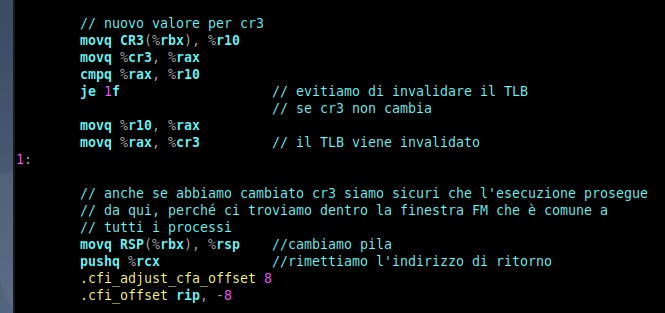
\includegraphics[scale=.9]{img/249.PNG}
%\end{center}
Nel codice evitiamo di sovrascrivere CR3 se già presente nel registro è uguale a quello che vogliamo porre. Lo facciamo per evitare di svuotare il TLB quando non necessario (ricordare cosa abbiamo detto sull'istruzione \emph{mov}): svuotarlo è un problema dal punto di vista delle prestazioni (centinaia di clock in più per una mossa che poteva essere evitata).


\section{Indirizzi virtuali e fisici nei file ELF}
\paragraph{Modulo sistema}
\begin{center}
	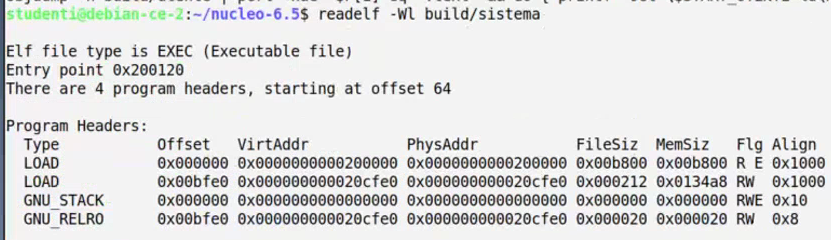
\includegraphics[scale=.75]{img/252.PNG}
\end{center}
Il modulo sistema viene collegato a indirizzi virtuali che sono effettivamente fisici. Il bootloader crea una traduzione identità, e gli cede il controllo. Grazie alla finestra sulla RAM continueremo ad utilizzare questi indirizzi. 


\paragraph{Modulo I/O} 
\begin{center}
	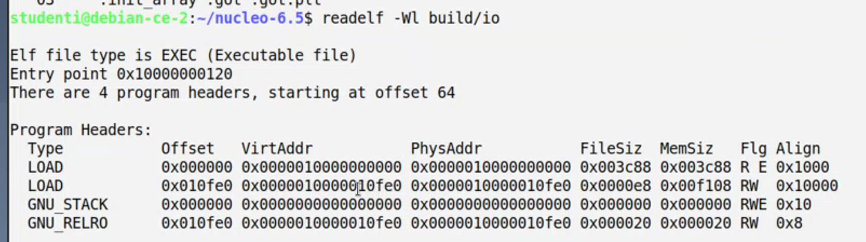
\includegraphics[scale=.70]{img/251.PNG}
\end{center}
Il modulo I/O sta da tutt'altra parte. Gli indirizzi sono molto più grandi e sono collocati nella parte dedicata al modulo I/O. 

\clearpage 
\paragraph{Modulo utente} 
\begin{center}
	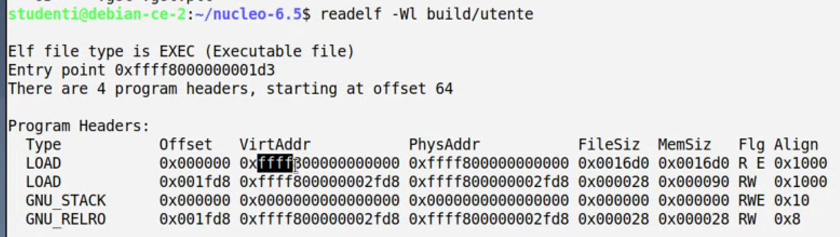
\includegraphics[scale=.75]{img/250.PNG}
\end{center}
Il modulo utente utilizza gli indirizzi oltre il buco (attenzione a \emph{ffff}).

\section{Strutture dati per la gestione dei frame}
\subsection{Descrittore di frame}
I frame sono descritti attraverso la struttura \emph{des$\_$frame}, il descrittore di frame.
\small 
\begin{verbatim}
	struct des_frame {
		union {
			// numero di entrate valide (se il frame contiene una tabella)
			natw nvalide;
			// lista di frame liberi (se il frame e' libero)
			natl prossimo_libero;
		};
	};
\end{verbatim}
\normalsize 
%\begin{center}
%	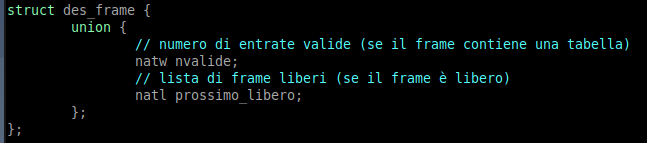
\includegraphics{img/253.PNG}
%\end{center}
\paragraph{Uso della union nel descrittore di frame}
Per ridurre lo spazio richiesto dall'array dei frame usiamo una \emph{union}: le informazioni nello struct non ci interessano mai in contemporanea.
\begin{itemize}
	\item \emph{nvalide} mi interessa quando il frame è occupato da una tabella, mi indica il numero di entrate valide in una tabella ($P=1$). Possiamo deallocare una tabella solo se tutti i $P$ sono uguali a zero (la cosa può servirmi al termine di un processo, devo verificare quali tabelle posso deallocare e quali no senza doverle scorrere per intero).
	\item \emph{prossimo$\_$libero} mi interessa solo quando il frame è libero, per sapere qual è il frame libero successivo.
\end{itemize}
\subsection{Array dei descrittori di frame e numero totale dei frame}
I descrittori di frame sono posti nel seguente array
\begin{verbatim}
	des_frame vdf[N_FRAME];
\end{verbatim}
dove \emph{N$\_$FRAME} è il numero di frame ($M1+M2$), che può essere determinato a priori dividendo la dimensione della memoria per la dimensione della pagina.
\begin{verbatim}
	natq const N_FRAME = MEM_TOT / DIM_PAGINA;
\end{verbatim}
Le costanti usate sono quelle della \emph{libce} introdotte qualche pagina indietro
\subsection{Lista dei frame liberi: testa e contatore}
Indice del primo frame libero (all'interno dell'array). 
\begin{verbatim}
	natq primo_frame_libero;
\end{verbatim}Con \emph{prossimo$\_$libero} andiamo a costruire una lista di frame liberi.
\paragraph{Numero di frame liberi}
Con la seguente variabile contiamo il numero di frame nella lista
\begin{verbatim}
	natq num_frame_liberi;
\end{verbatim}

\subsection{Numero dei frame in $M1$ e in $M2$} 
Nelle seguenti variabili poniamo il numero di frame riservati per $M1$ e il numero di frame riservati per $M2$
\begin{verbatim}
	natq N_M1;
	natq N_M2;
\end{verbatim}

\section{Funzioni di utilità per il contatore \emph{nvalide} nel \emph{des$\_$frame}}
%\begin{center}
%	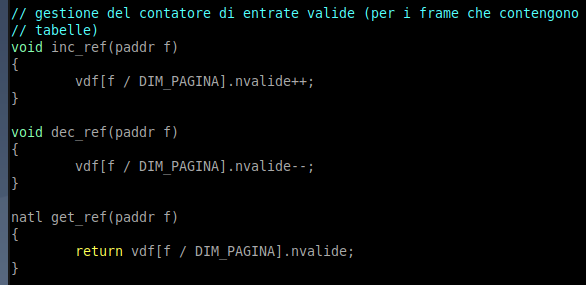
\includegraphics{img/256.PNG}
%\end{center}
Le seguenti funzioni di utilità manipolano il contatore \emph{nvalide} in un descrittore di frame. 
\small 
\begin{verbatim}
	void inc_ref(paddr f) {
		vdf[f / DIM_PAGINA].nvalide++;
	}
	
	void dec_ref(paddr f) {
		vdf[f / DIM_PAGINA].nvalide--;
	}
	
	natl get_ref(paddr f) {
		return vdf[f / DIM_PAGINA].nvalide;
	}
\end{verbatim}
\normalsize 
Esse richiedono in ingresso un indirizzo fisico relativo al  frame.
\begin{itemize}
	\item \emph{inc$\_$ref} incrementa il contatore delle entrate valide.
	\item \emph{dec$\_$ref} decrementa il contatore delle entrate valide.
	\item \emph{get$\_$ref} restituisce il valore del contatore delle entrate valide.
\end{itemize}

\section{Funzioni per la gestione della paginazione}
\subsection{Funzione per l'occupazione di un frame libero (\emph{alloca$\_$frame})}
%\begin{center}
%	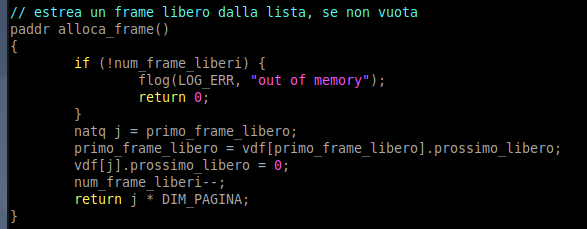
\includegraphics{img/254.PNG}
%\end{center}
\small 
\begin{verbatim}
	// estrea un frame libero dalla lista, se non vuota
	paddr alloca_frame() {
		if (!num_frame_liberi) {
			flog(LOG_ERR, "out of memory");
			return 0;
		}
		natq j = primo_frame_libero;
		primo_frame_libero = vdf[primo_frame_libero].prossimo_libero;
		vdf[j].prossimo_libero = 0;
		num_frame_liberi--;
		
		return j * DIM_PAGINA;
	}
\end{verbatim}
\normalsize 
\begin{itemize}
	\item Controllo se la memoria non sia tutta occupata attraverso il contatore \emph{num$\_$frame$\_$liberi}. Se tutti i frame sono occupati segnalo con \emph{flog} e mi fermo restituendo $0$.
	\item Se la memoria non è occupata prendo la testa della lista dei frame liberi, \emph{primo$\_$frame$\_$libero} e ne restituisco l'indirizzo fisico della base. L'indirizzo fisico si calcola moltiplicando l'indice della testa per \emph{DIM$\_$PAGINA}.
	\item Modifico il puntatore \emph{primo$\_$frame$\_$libero}: abbiamo rimosso la testa della lista.  
	\item Modifico anche il puntatore \emph{prossimo$\_$libero} nel descrittore stesso, azzerandolo (non fa più parte della lista).
	\item Decremento il numero di frame liberi (\emph{num$\_$frame$\_$liberi}).
\end{itemize}
\[\boxed{\text{La funzione si presta bene come \emph{getpaddr} nella funzione \emph{map}, affrontata poco più avanti.}}\]
\subsection{Funzione per il rilascio di un frame occupato (\emph{rilascia$\_$frame})}
\small 
\begin{verbatim}
	// rende di nuovo libera il frame descritto da df
	void rilascia_frame(paddr f) {
		natq j = f / DIM_PAGINA;
		if (j < N_M1) {
			panic("tentativo di rilasciare un frame di M1");
		}
		vdf[j].prossimo_libero = primo_frame_libero;
		primo_frame_libero = j;
		num_frame_liberi++;
	}
\end{verbatim}
\normalsize 
%\begin{center}
%	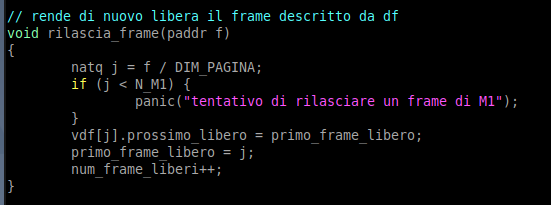
\includegraphics{img/255.PNG}
%\end{center}
\begin{itemize}
	\item Quando vogliamo rilasciare un frame passiamo in ingresso l'indirizzo fisico della base del frame.
	\item Si calcola il numero di frame dividendo l'indirizzo per \emph{DIM$\_$PAGINA}. 
	\item Se il frame risulta appartenente ad $M1$ blocco tutto chiamando la \emph{panic}.
	\item Colloco il descrittore rilasciato nella lista dei frame liberi. Non ha senso mettere il descrittore in un posto specifico (come invece facevamo coi processi, \emph{precedenza}): grazie alla MMU non ci fa nessuna differenza avere un frame o un altro. Il rilascio più semplice possibile consiste nel mettere in testa il descrittore del frame rilasciato.
\end{itemize}
\[\boxed{\text{La funzione si presta bene come \emph{putpaddr} nella funzione \emph{unmap} (l'opposto della \emph{map}).}}\]
\subsection{Allocazione della tabella con \emph{alloca$\_$tab} (usa \emph{alloca$\_$frame})}
%\begin{center}
%	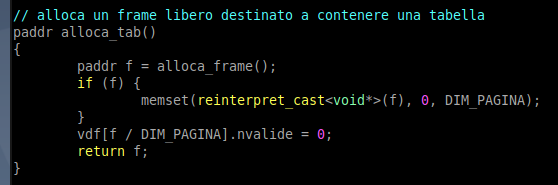
\includegraphics{img/258.PNG}
%\end{center}
\small 
\begin{verbatim}
	// alloca un frame libero destinato a contenere una tabella
	paddr alloca_tab() {
		paddr f = alloca_frame();
		if (f) {
			memset(reinterpret_cast<void*>(f), 0, DIM_PAGINA);
		}
		vdf[f / DIM_PAGINA].nvalide = 0;
		return f;
	}
\end{verbatim}
\normalsize 
\begin{itemize}
	\item Allocare una tabella significa allocare un frame. Quindi chiamo la \emph{alloca$\_$frame}.
	\item Il valore restituito dalla \emph{alloca$\_$frame} è $0$ se non è stato possibile allocare il frame. Se l'allocazione ha successo chiamo la \emph{memset}, con cui resetto il contenuto del frame (scrive dentro l'indirizzo il byte $0$ per \emph{DIM$\_$PAGINA} volte).
	\item Pongo a $0$ il contatore \emph{nvalide}.
	\item Restituisco l'indirizzo indicato dalla \emph{alloca$\_$frame}.
\end{itemize} 
\subsection{Rilascio della tabella con \emph{rilascia$\_$tab} (usa \emph{rilascia$\_$frame})}
\small 
\begin{verbatim}
	// dealloca un frame che contiene una tabella, controllando che non contenga entrate valide
	void rilascia_tab(paddr f) {
		if (int n = get_ref(f)) {
			flog(LOG_ERR, "tentativo di deallocare la tabella %x con %d entrate valide", f, n);
			panic("errore interno");
		}
		rilascia_frame(f);
	}
\end{verbatim}
\normalsize 
%\begin{center}
%	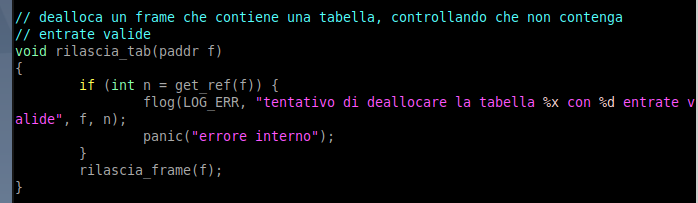
\includegraphics{img/259.PNG}
%\end{center}
\begin{itemize}
	\item Quando rilasciamo una tabella dobbiamo controllare che non sia utilizzata con la funzione di utilità \emph{get$\_$ref}.
	\item Se il controllo ci dice che la tabella non è utilizzata allora rilasciamo il frame chiamando la \emph{rilascia$\_$frame}.
\end{itemize}

\subsection{Settaggio dell'entrata di una tabella con \emph{set$\_$entry}}
\small 
\begin{verbatim}
	// setta l'entrata j-esima della tabella 'tab' con il valore 'se'.
	// Si preoccupa di aggiustare opporutinamente il contatore delle
	// entrate valide.
	void set_entry(paddr tab, natl j, tab_entry se) {
		tab_entry& de = get_entry(tab, j);
		if ((se & BIT_P) && !(de & BIT_P)) {
			inc_ref(tab);
		} else if (!(se & BIT_P) && (de & BIT_P)) {
			dec_ref(tab);
		}
		de = se;
	}
\end{verbatim}
\normalsize
%\begin{center}
%	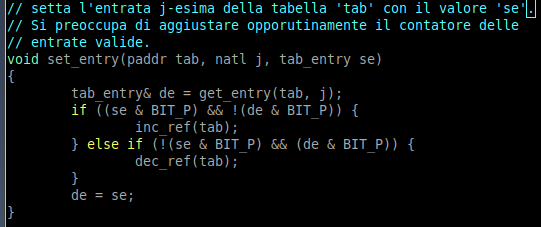
\includegraphics{img/260.PNG}
%\end{center}
\begin{itemize}
	\item La funzione richiede l'indirizzo fisico della tabella \emph{tab}, l'indice \emph{j} dell'entrata, e l'entrata \emph{se}.
	\item Recuperiamo il contenuto attuale dell'entrata \emph{j} nella tabella \emph{tab} con la funzione \emph{get$\_$entry}.
	\item Gestiamo l'incremento di \emph{nvalide} nel descrittore di frame.
	\begin{itemize}
		\item Se nella nuova c'è il bit $P=1$ e nella vecchia $P=0$ incrementiamo con \emph{inc$\_$ref}.
		\item Se nella nuova c'è il bit $P=0$ e nella vecchia $P=1$ decrementiamo con \emph{dec$\_$ref}.
	\end{itemize}
	\item Concludiamo sostituendo l'entrata vecchia con la nuova.
\end{itemize}
\subsection{Copia di descrittori da una tabella a un'altra (\emph{copy$\_$des})}
\small 
\begin{verbatim}
	// copia 'n' descrittori a partire da quello di indice 'i' dalla
	// tabella di indirizzo 'src' in quella di indirizzo 'dst'
	void copy_des(paddr src, paddr dst, natl i, natl n) {
		for (natl j = i; j < i + n && j < 512; j++) {
			tab_entry se = get_entry(src, j);
			set_entry(dst, j, se);
		}
	}
\end{verbatim}
\normalsize 
%\begin{center}
%	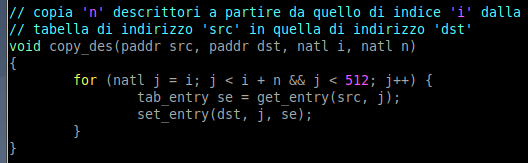
\includegraphics{img/261.PNG}
%\end{center}
\begin{itemize}
	\item Con la funzione possiamo copiare entrate da una tabella \emph{src} alla \emph{dst}, ne copio \emph{n} a partire dall'entrata $i-$esima.
	\item Faccio un for, ogni volta leggo l'entrata sorgente con \emph{get$\_$entry} e setto l'entrata destinataria con \emph{set$\_$entry}. L'ultima funzione mi gestisce anche l'aggiornamento del contatore \emph{nvalide}.
\end{itemize}
\subsection{Settaggio di descrittori uguali in una tabella (\emph{set$\_$des})}
\small 
\begin{verbatim}
	// setta 'n' descrittori a partire da quello di indice 'i' nella
	// tabella di indirizzo 'dst' con valore 'e'
	void set_des(paddr dst, natl i, natl n, tab_entry e) {
		for (natl j = i; j < i + n && j < 512; j++) {
			set_entry(dst, j, e);
		}
	}
\end{verbatim}
\normalsize 
%\begin{center}
%	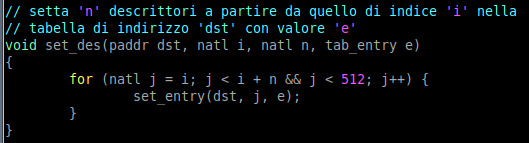
\includegraphics{img/262.PNG}
%\end{center}
\begin{itemize}
	\item Imposto $n$ entrate della tabella \emph{dst}, tutte uguali ad \emph{e}, a partire dalla $i-$esima.
	\item Nel for utilizziamo solo la funzione di utilità \emph{set$\_$entry}, con cui gestisco anche l'aggiornamento del contatore \emph{nvalide}.
\end{itemize}
\clearpage 

\section{Funzione \emph{map}}
\[\boxed{\text{La funzione più utile di tutte (cit.).}}\]
\begin{verbatim}
	template<typename T>
	vaddr map(paddr tab, vaddr begin, vaddr end, natl flags, T getpaddr, int ps_lvl = 1);
\end{verbatim}
\paragraph{Scopo} La funzione crea una traduzione per tutti gli indirizzi dell'intervallo $[\text{begin}, \text{end}[$ nel  trie di radice \emph{tab}. Ogni traduzione dovrà avere i flag \emph{flags} indicati. Opzionalmente possiamo settare il \emph{page size} uguale ad $1$ in un livello diverso dal livello $1$: indicando come \emph{page size level} $2$ posso creare pagine da 2 MB, ad esempio. Con \emph{getpaddr} indichiamo l'indirizzo fisico corrispondente.
\paragraph{Vediamo}
\begin{itemize}
	\item \textbf{Il \emph{typename} e il parametro di ingresso \emph{getpaddr}}.
	
	Vogliamo creare una traduzione per un intervallo di indirizzi. Molte delle cose da fare non dipendono da cosa vogliamo far corrispondere a questi indirizzi. La funzione è stata resa generica, in modo da utilizzarla in più situazioni possibili: non sa lei direttamente quali indirizzi fisici associare a quelli virtuale. Per fare questa associazione ricorriamo all'oggetto \emph{getpaddr}, il cui tipo \emph{T} è stabilito dal \emph{typename} (studiato ad \emph{Algoritmi e Strutture dati}).
	
	All'interno del codice della funzione troverò a un certo punto il seguente assegnamento
	\begin{verbatim}
		new_f = getpaddr(v);
	\end{verbatim}
	esso mi restituisce, dato l'indirizzo virtuale \emph{v}, il corrispondente indirizzo fisico. Dalla sintassi deduciamo che \emph{getpaddr} funziona con:
	\begin{itemize}
		\item puntatori a funzione;
		\item classi dove ridefiniamo l'operatore parentesi (la classe può ricordarsi anche altre cose).
	\end{itemize}
	In tutti gli altri casi il compilatore segnala errore.
	\item \textbf{Verifica dei parametri di ingresso}.
	\begin{itemize}
		\item \textbf{Indirizzi \emph{begin} e \emph{end}}. 
		
		La prima cosa che dobbiamo fare nel codice è verificare che \emph{begin} ed \emph{end} siano validi. Calcoliamo la dimensione della regione e verifichiamo che l'allineamento alle pagine
		\begin{verbatim}
			natq dr = dim_region(ps_lvl - 1);
		\end{verbatim}
		\begin{itemize}
			\item  Verifico che \emph{begin} sia allineato alle pagine di livello \emph{ps$\_$lvl}.
			\begin{verbatim}
				if(begin & (dr - 1)) ...
			\end{verbatim}
			La condizione risulta vera se esiste almeno un bit tra i meno significativi che non è nullo (per avere l'allineamento rispetto a una certa dimensione i primi bit devono essere nulli).
			\item  Verifico che \emph{end} sia allineato alle pagine di livello \emph{ps$\_$lvl}. 
			\begin{verbatim}
				if(end & (dr - 1)) ...	\end{verbatim}
			Valgono gli stessi ragionamenti fatti con \emph{begin}.
		\end{itemize}
		\small
		\begin{verbatim}
			natq dr = dim_region(ps_lvl - 1);
			if (begin & (dr - 1)) {
				flog(LOG_ERR, "begin=%p non allineato alle pagine di livello %d", begin, ps_lvl);
				panic("chiamata di map() non valida");
			}
			if (end & (dr - 1)) {
				flog(LOG_ERR, "end=%p non allineato alle pagine di livello %d", end, ps_lvl);
				panic("chiamata di map() non valida");
			}
		\end{verbatim}
		\normalsize 
		\item \textbf{Parametro di ingresso \emph{flags}}. 
		
		\noindent Verifico che gli unici flag modificati siano tra RW, US, PWT e PCD. Prendo le relative maschere (già viste nelle costanti), le unisco con l'operatore OR, e nego il risultato. Ottengo una maschera dove sono uguali ad $1$ tutti i bit tranne quelli di cui è consentita la modifica.
		\small
		\begin{verbatim}
			if (flags & ~(BIT_RW|BIT_US|BIT_PWT|BIT_PCD)) {
				panic("flags contiene bit non validi (ammessi RW, US, PWT e PCD)");
			}
		\end{verbatim}
		\normalsize
		
		\item \textbf{\emph{ps$\_$lev}}.
		
		\noindent Verifico che \emph{ps$\_$lvl} sia stato impostato correttamente:
		\begin{itemize}
			\item Non deve essere minore di $1$
			\item Non deve essere maggiore del livello massimo \emph{MAX$\_$PS$\_$LVL}
		\end{itemize} 
		\small
		\begin{verbatim}
			if (ps_lvl < 1 || ps_lvl > MAX_PS_LVL) {
				flog(
				LOG_ERR, 
				"ps_lvl %d non ammesso (deve essere compreso tra 2 e %d)", 
				ps_lvl, 
				MAX_PS_LVL
				);
				panic("chiamata di map() non valida");
			}
		\end{verbatim}
		\normalsize
	\end{itemize} 
	
	\item \textbf{Uso della funzione}.
	
	Usiamo la funzione per creare tutte le parti dello spazio di indirizzamento. 
	\begin{itemize}
		\item Quelle condivise sono le stesse in ogni processo, dunque la loro traduzione può essere fatta all'avvio. 
		\begin{center}
			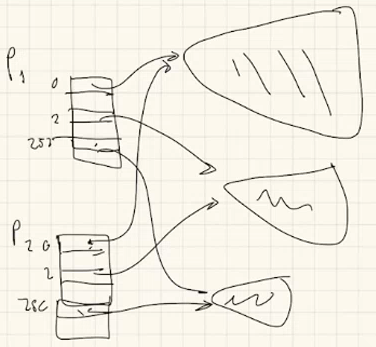
\includegraphics[scale=.75]{img/265.PNG}
		\end{center}
		Abbiamo sotto-alberi condivisi tra più alberi. Li creiamo inizialmente per il processo \emph{dummy} (processo che è sempre vivo). 
		\item Ogni volta che creiamo un processo ci limitiamo a creare solo le parti di albero relative esclusivamente  a quel processo. Per quanto riguarda le parti condivise ci limitiamo a porre i relativi indirizzi fisici nella tabella di livello $4$ (non dobbiamo ricreare queste parti nuovamente).
	\end{itemize}
	All'avvio del nucleo, dopo l'inizializzazione dell'APIC, abbiamo
	\begin{center}
		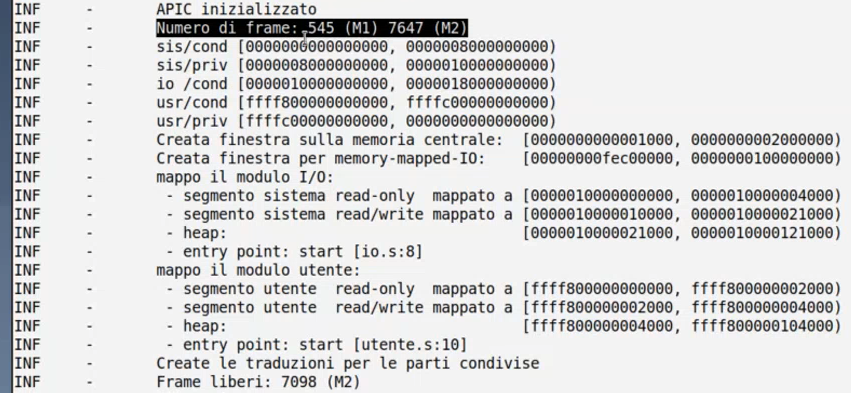
\includegraphics[scale=.8]{img/266.PNG}
	\end{center}
	\begin{itemize}
		\item Indico il numero di frame in $M1$ e in $M2$ (numero stabilito a priori).
		\item Calcolo e stampo gli indirizzi virtuali estremi dei vari intervalli definiti nello spazio di indirizzamento: sis/cond, sis/priv, io/cond, usr/cond, usr/priv.
		\item Creo le varie parti condivise una volta per tutte: 
		\begin{itemize}
			\item la finestra sulla parte centrale (solo sulla RAM, di grandezza variabile),
			\item la finestra sul \emph{memory mapped I/O},
			\item il modulo I/O,
			\item il modulo utente.
		\end{itemize}
		Quando il controllo viene passato al modulo sistema questo interpreta il file ELF e vede a che indirizzi virtuali devono andare le varie parti del file ELF.
	\end{itemize}
\end{itemize} 